\documentclass[]{book}
\usepackage{lmodern}
\usepackage{amssymb,amsmath}
\usepackage{ifxetex,ifluatex}
\usepackage{fixltx2e} % provides \textsubscript
\ifnum 0\ifxetex 1\fi\ifluatex 1\fi=0 % if pdftex
  \usepackage[T1]{fontenc}
  \usepackage[utf8]{inputenc}
\else % if luatex or xelatex
  \ifxetex
    \usepackage{mathspec}
  \else
    \usepackage{fontspec}
  \fi
  \defaultfontfeatures{Ligatures=TeX,Scale=MatchLowercase}
\fi
% use upquote if available, for straight quotes in verbatim environments
\IfFileExists{upquote.sty}{\usepackage{upquote}}{}
% use microtype if available
\IfFileExists{microtype.sty}{%
\usepackage{microtype}
\UseMicrotypeSet[protrusion]{basicmath} % disable protrusion for tt fonts
}{}
\usepackage[margin=1in]{geometry}
\usepackage{hyperref}
\hypersetup{unicode=true,
            pdftitle={bdchecks User Guide},
            pdfauthor={Authors: Tomer Gueta and Povilas Gibas},
            pdfborder={0 0 0},
            breaklinks=true}
\urlstyle{same}  % don't use monospace font for urls
\usepackage{natbib}
\bibliographystyle{apalike}
\usepackage{color}
\usepackage{fancyvrb}
\newcommand{\VerbBar}{|}
\newcommand{\VERB}{\Verb[commandchars=\\\{\}]}
\DefineVerbatimEnvironment{Highlighting}{Verbatim}{commandchars=\\\{\}}
% Add ',fontsize=\small' for more characters per line
\usepackage{framed}
\definecolor{shadecolor}{RGB}{248,248,248}
\newenvironment{Shaded}{\begin{snugshade}}{\end{snugshade}}
\newcommand{\KeywordTok}[1]{\textcolor[rgb]{0.13,0.29,0.53}{\textbf{#1}}}
\newcommand{\DataTypeTok}[1]{\textcolor[rgb]{0.13,0.29,0.53}{#1}}
\newcommand{\DecValTok}[1]{\textcolor[rgb]{0.00,0.00,0.81}{#1}}
\newcommand{\BaseNTok}[1]{\textcolor[rgb]{0.00,0.00,0.81}{#1}}
\newcommand{\FloatTok}[1]{\textcolor[rgb]{0.00,0.00,0.81}{#1}}
\newcommand{\ConstantTok}[1]{\textcolor[rgb]{0.00,0.00,0.00}{#1}}
\newcommand{\CharTok}[1]{\textcolor[rgb]{0.31,0.60,0.02}{#1}}
\newcommand{\SpecialCharTok}[1]{\textcolor[rgb]{0.00,0.00,0.00}{#1}}
\newcommand{\StringTok}[1]{\textcolor[rgb]{0.31,0.60,0.02}{#1}}
\newcommand{\VerbatimStringTok}[1]{\textcolor[rgb]{0.31,0.60,0.02}{#1}}
\newcommand{\SpecialStringTok}[1]{\textcolor[rgb]{0.31,0.60,0.02}{#1}}
\newcommand{\ImportTok}[1]{#1}
\newcommand{\CommentTok}[1]{\textcolor[rgb]{0.56,0.35,0.01}{\textit{#1}}}
\newcommand{\DocumentationTok}[1]{\textcolor[rgb]{0.56,0.35,0.01}{\textbf{\textit{#1}}}}
\newcommand{\AnnotationTok}[1]{\textcolor[rgb]{0.56,0.35,0.01}{\textbf{\textit{#1}}}}
\newcommand{\CommentVarTok}[1]{\textcolor[rgb]{0.56,0.35,0.01}{\textbf{\textit{#1}}}}
\newcommand{\OtherTok}[1]{\textcolor[rgb]{0.56,0.35,0.01}{#1}}
\newcommand{\FunctionTok}[1]{\textcolor[rgb]{0.00,0.00,0.00}{#1}}
\newcommand{\VariableTok}[1]{\textcolor[rgb]{0.00,0.00,0.00}{#1}}
\newcommand{\ControlFlowTok}[1]{\textcolor[rgb]{0.13,0.29,0.53}{\textbf{#1}}}
\newcommand{\OperatorTok}[1]{\textcolor[rgb]{0.81,0.36,0.00}{\textbf{#1}}}
\newcommand{\BuiltInTok}[1]{#1}
\newcommand{\ExtensionTok}[1]{#1}
\newcommand{\PreprocessorTok}[1]{\textcolor[rgb]{0.56,0.35,0.01}{\textit{#1}}}
\newcommand{\AttributeTok}[1]{\textcolor[rgb]{0.77,0.63,0.00}{#1}}
\newcommand{\RegionMarkerTok}[1]{#1}
\newcommand{\InformationTok}[1]{\textcolor[rgb]{0.56,0.35,0.01}{\textbf{\textit{#1}}}}
\newcommand{\WarningTok}[1]{\textcolor[rgb]{0.56,0.35,0.01}{\textbf{\textit{#1}}}}
\newcommand{\AlertTok}[1]{\textcolor[rgb]{0.94,0.16,0.16}{#1}}
\newcommand{\ErrorTok}[1]{\textcolor[rgb]{0.64,0.00,0.00}{\textbf{#1}}}
\newcommand{\NormalTok}[1]{#1}
\usepackage{longtable,booktabs}
\usepackage{graphicx,grffile}
\makeatletter
\def\maxwidth{\ifdim\Gin@nat@width>\linewidth\linewidth\else\Gin@nat@width\fi}
\def\maxheight{\ifdim\Gin@nat@height>\textheight\textheight\else\Gin@nat@height\fi}
\makeatother
% Scale images if necessary, so that they will not overflow the page
% margins by default, and it is still possible to overwrite the defaults
% using explicit options in \includegraphics[width, height, ...]{}
\setkeys{Gin}{width=\maxwidth,height=\maxheight,keepaspectratio}
\IfFileExists{parskip.sty}{%
\usepackage{parskip}
}{% else
\setlength{\parindent}{0pt}
\setlength{\parskip}{6pt plus 2pt minus 1pt}
}
\setlength{\emergencystretch}{3em}  % prevent overfull lines
\providecommand{\tightlist}{%
  \setlength{\itemsep}{0pt}\setlength{\parskip}{0pt}}
\setcounter{secnumdepth}{5}
% Redefines (sub)paragraphs to behave more like sections
\ifx\paragraph\undefined\else
\let\oldparagraph\paragraph
\renewcommand{\paragraph}[1]{\oldparagraph{#1}\mbox{}}
\fi
\ifx\subparagraph\undefined\else
\let\oldsubparagraph\subparagraph
\renewcommand{\subparagraph}[1]{\oldsubparagraph{#1}\mbox{}}
\fi

%%% Use protect on footnotes to avoid problems with footnotes in titles
\let\rmarkdownfootnote\footnote%
\def\footnote{\protect\rmarkdownfootnote}

%%% Change title format to be more compact
\usepackage{titling}

% Create subtitle command for use in maketitle
\newcommand{\subtitle}[1]{
  \posttitle{
    \begin{center}\large#1\end{center}
    }
}

\setlength{\droptitle}{-2em}

  \title{\texttt{bdchecks} User Guide}
    \pretitle{\vspace{\droptitle}\centering\huge}
  \posttitle{\par}
    \author{Authors: Tomer Gueta and Povilas Gibas}
    \preauthor{\centering\large\emph}
  \postauthor{\par}
      \predate{\centering\large\emph}
  \postdate{\par}
    \date{built on 2018-10-16}

\usepackage{booktabs}

\usepackage{amsthm}
\newtheorem{theorem}{Theorem}[chapter]
\newtheorem{lemma}{Lemma}[chapter]
\theoremstyle{definition}
\newtheorem{definition}{Definition}[chapter]
\newtheorem{corollary}{Corollary}[chapter]
\newtheorem{proposition}{Proposition}[chapter]
\theoremstyle{definition}
\newtheorem{example}{Example}[chapter]
\theoremstyle{definition}
\newtheorem{exercise}{Exercise}[chapter]
\theoremstyle{remark}
\newtheorem*{remark}{Remark}
\newtheorem*{solution}{Solution}
\begin{document}
\maketitle

{
\setcounter{tocdepth}{1}
\tableofcontents
}
\chapter*{Introduction}\label{introduction}
\addcontentsline{toc}{chapter}{Introduction}

\texttt{bdchecks} supplies a Shiny app and a set of functions to perform
and manage various data checks for biodiversity data. \texttt{bdchecks}
is part of the \texttt{bdverse}-- a collection of tools, that form a
general framework for facilitating biodiversity science in R.

\begin{figure}
\centering
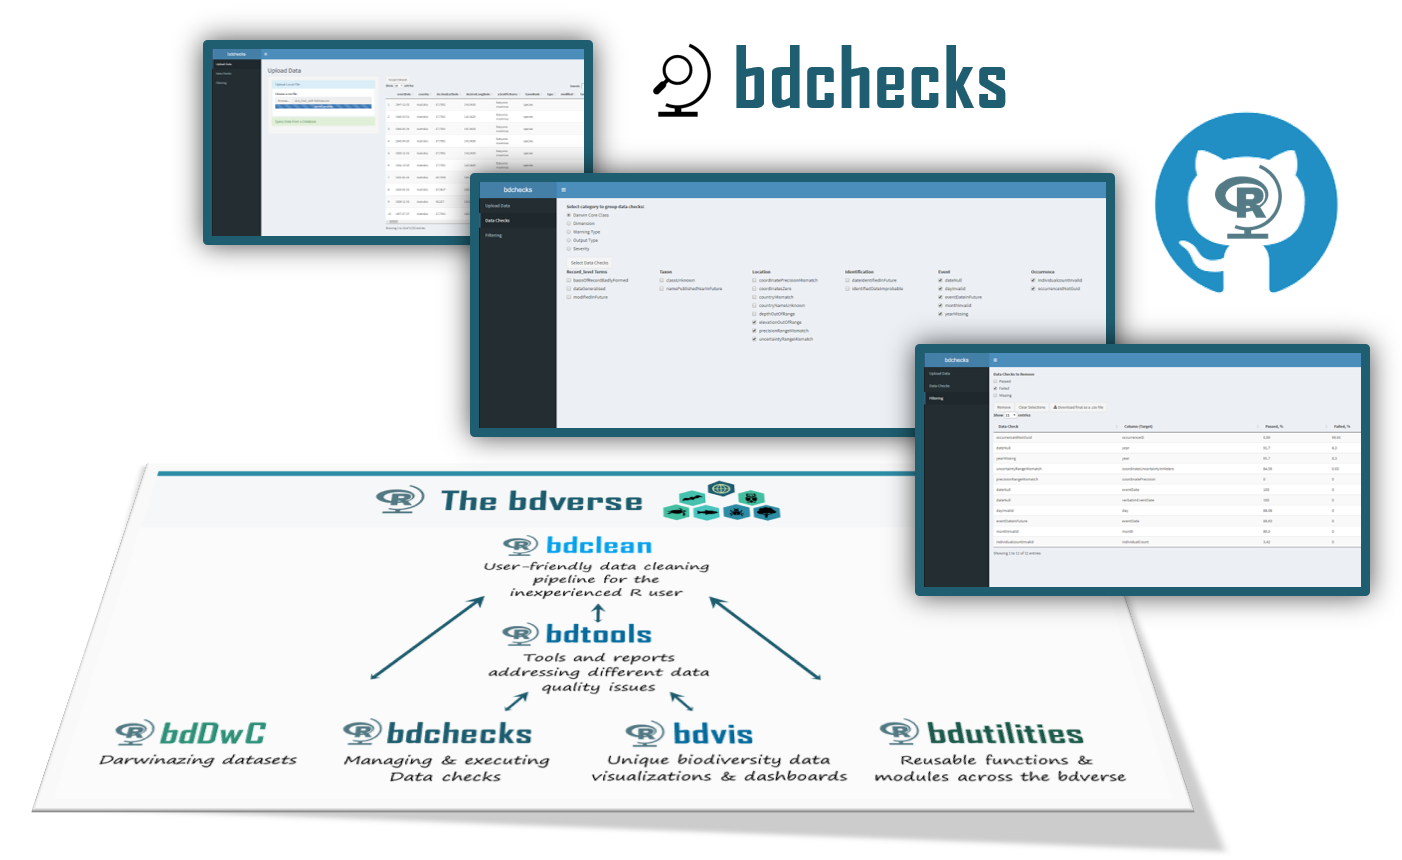
\includegraphics{img/bdchecks_bdverse.png}
\caption{bdchecks in the bdverse}
\end{figure}

\subsubsection*{What are biodiversity data
checks?}\label{what-are-biodiversity-data-checks}
\addcontentsline{toc}{subsubsection}{What are biodiversity data checks?}

Data checks can include format checks, completeness checks,
reasonableness checks, limit checks, etc. These processes usually result
in flagging, documenting, and subsequent correcting or eliminating of
suspect records. The checks must be specifically tailored around the
structure of the data at hand, in our case, the Darwin Core standard.
Ideally, a data check needs to hold its functionality and relevant
metadata.

\subsubsection*{\texorpdfstring{What \texttt{bdchecks} can do for
you?}{What bdchecks can do for you?}}\label{what-bdchecks-can-do-for-you}
\addcontentsline{toc}{subsubsection}{What \texttt{bdchecks} can do for
you?}

\texttt{bdchecks} offers various features for various R users:

\begin{itemize}
\tightlist
\item
  Using the Shiny app \textbf{inexperienced R users} can easily perform
  all data check and can easily filter the data accordingly. See
  \protect\hyperlink{the-shiny-app}{The shiny app} section.
\item
  \textbf{Experienced R users} can perform all data checks by utilizing
  few R functions form the command line or within an R script. See
  \protect\hyperlink{command-line-operations}{Command line operations}
  section.
\item
  \textbf{Advanced R users} can even edit, add and manage their own
  collection of data checks, quite easily so. See
  \protect\hyperlink{data-checks-yaml-file}{Data checks YAML file}
  section.
\end{itemize}

\subsubsection*{Fundings}\label{fundings}
\addcontentsline{toc}{subsubsection}{Fundings}

\begin{figure}
\centering

\includegraphics{img/ISF.png}
\caption{}
\end{figure}

\href{https://summerofcode.withgoogle.com/\%20target=\%22_blank\%22}{
\includegraphics{img/GSoC.png}}

\begin{itemize}
\tightlist
\item
  See the GSoC project idea page
\end{itemize}

\chapter{\texorpdfstring{Installing
\texttt{bdchecks}}{Installing bdchecks}}\label{installing-bdchecks}

\section{Development version from
GitHub}\label{development-version-from-github}

Windows users install
\href{https://cran.r-project.org/bin/windows/Rtools/}{Rtools} first.

\begin{Shaded}
\begin{Highlighting}[]
\KeywordTok{install.packages}\NormalTok{(}\StringTok{"devtools"}\NormalTok{)}
\NormalTok{devtools}\OperatorTok{::}\KeywordTok{install_github}\NormalTok{(}\StringTok{"bd-R/bdchecks"}\NormalTok{)}
\end{Highlighting}
\end{Shaded}

\section{\texorpdfstring{{Very soon: a stable version from
CRAN}}{Very soon: a stable version from CRAN}}\label{very-soon-a-stable-version-from-cran}

\begin{Shaded}
\begin{Highlighting}[]
\KeywordTok{install.packages}\NormalTok{(}\StringTok{"bdchecks"}\NormalTok{)}
\end{Highlighting}
\end{Shaded}

\section{Possible installation problems \&
solutions}\label{possible-installation-problems-solutions}

\textbf{{{[} TBA {]}}}

\subsection{???}\label{section}

TBA

\subsection{????}\label{section-1}

TBA***

\hypertarget{the-shiny-app}{\chapter{The shiny
app}\label{the-shiny-app}}

\begin{center}\rule{0.5\linewidth}{\linethickness}\end{center}

\section{Launching the app}\label{launching-the-app}

\begin{Shaded}
\begin{Highlighting}[]
\KeywordTok{library}\NormalTok{(bdchecks) }\CommentTok{# Uplaod package library}
\KeywordTok{runbdchecks}\NormalTok{() }\CommentTok{# Launch the app}
\end{Highlighting}
\end{Shaded}

\section{Data upload}\label{data-upload}

\subsection{From a local file}\label{from-a-local-file}

A CSV file or a Darwin Core Archive (DwC-A) zip file can be uploaded.

\begin{figure}
\centering
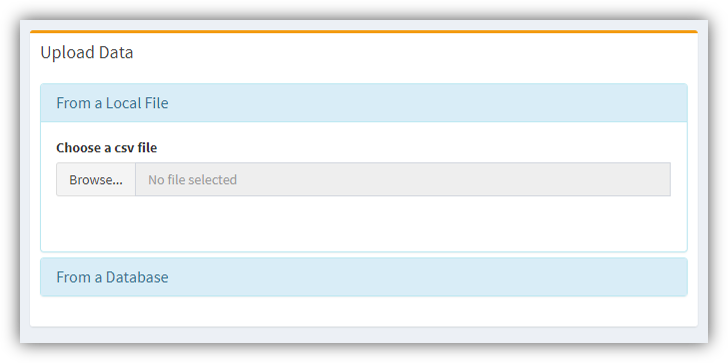
\includegraphics{img/bdchecks_Up-local_file.png}
\caption{Data upload from a local file}
\end{figure}

\subsection{From an online database}\label{from-an-online-database}

Also, data can be retrieved directly from various online biodiversity
databases. You need only to:

\begin{itemize}
\tightlist
\item
  Select the database
\item
  Specify the desired scientific name.
\item
  Specify the number of records (upper limit of 50,000).
\item
  Check the box if records must have coordinates.
\item
  Wait for data to be downloaded.
\end{itemize}

\begin{figure}
\centering
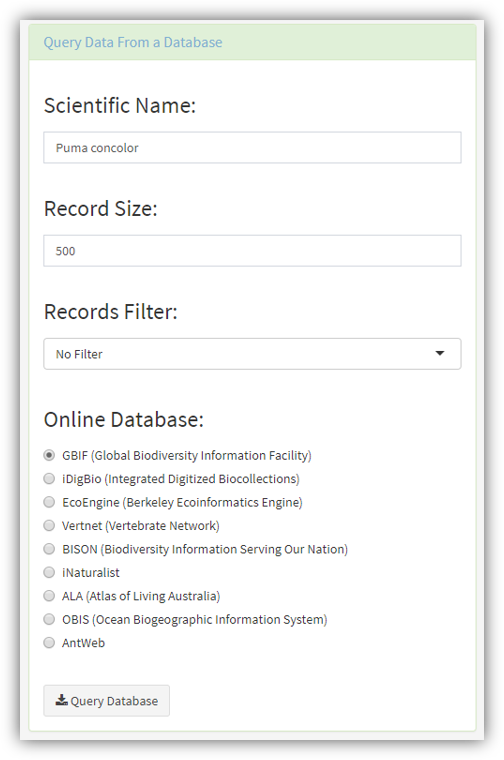
\includegraphics{img/bdchecks_Up-database.png}
\caption{Data upload from online biodiversity databases}
\end{figure}

\subsection{Accept dataset}\label{accept-dataset}

\begin{figure}
\centering
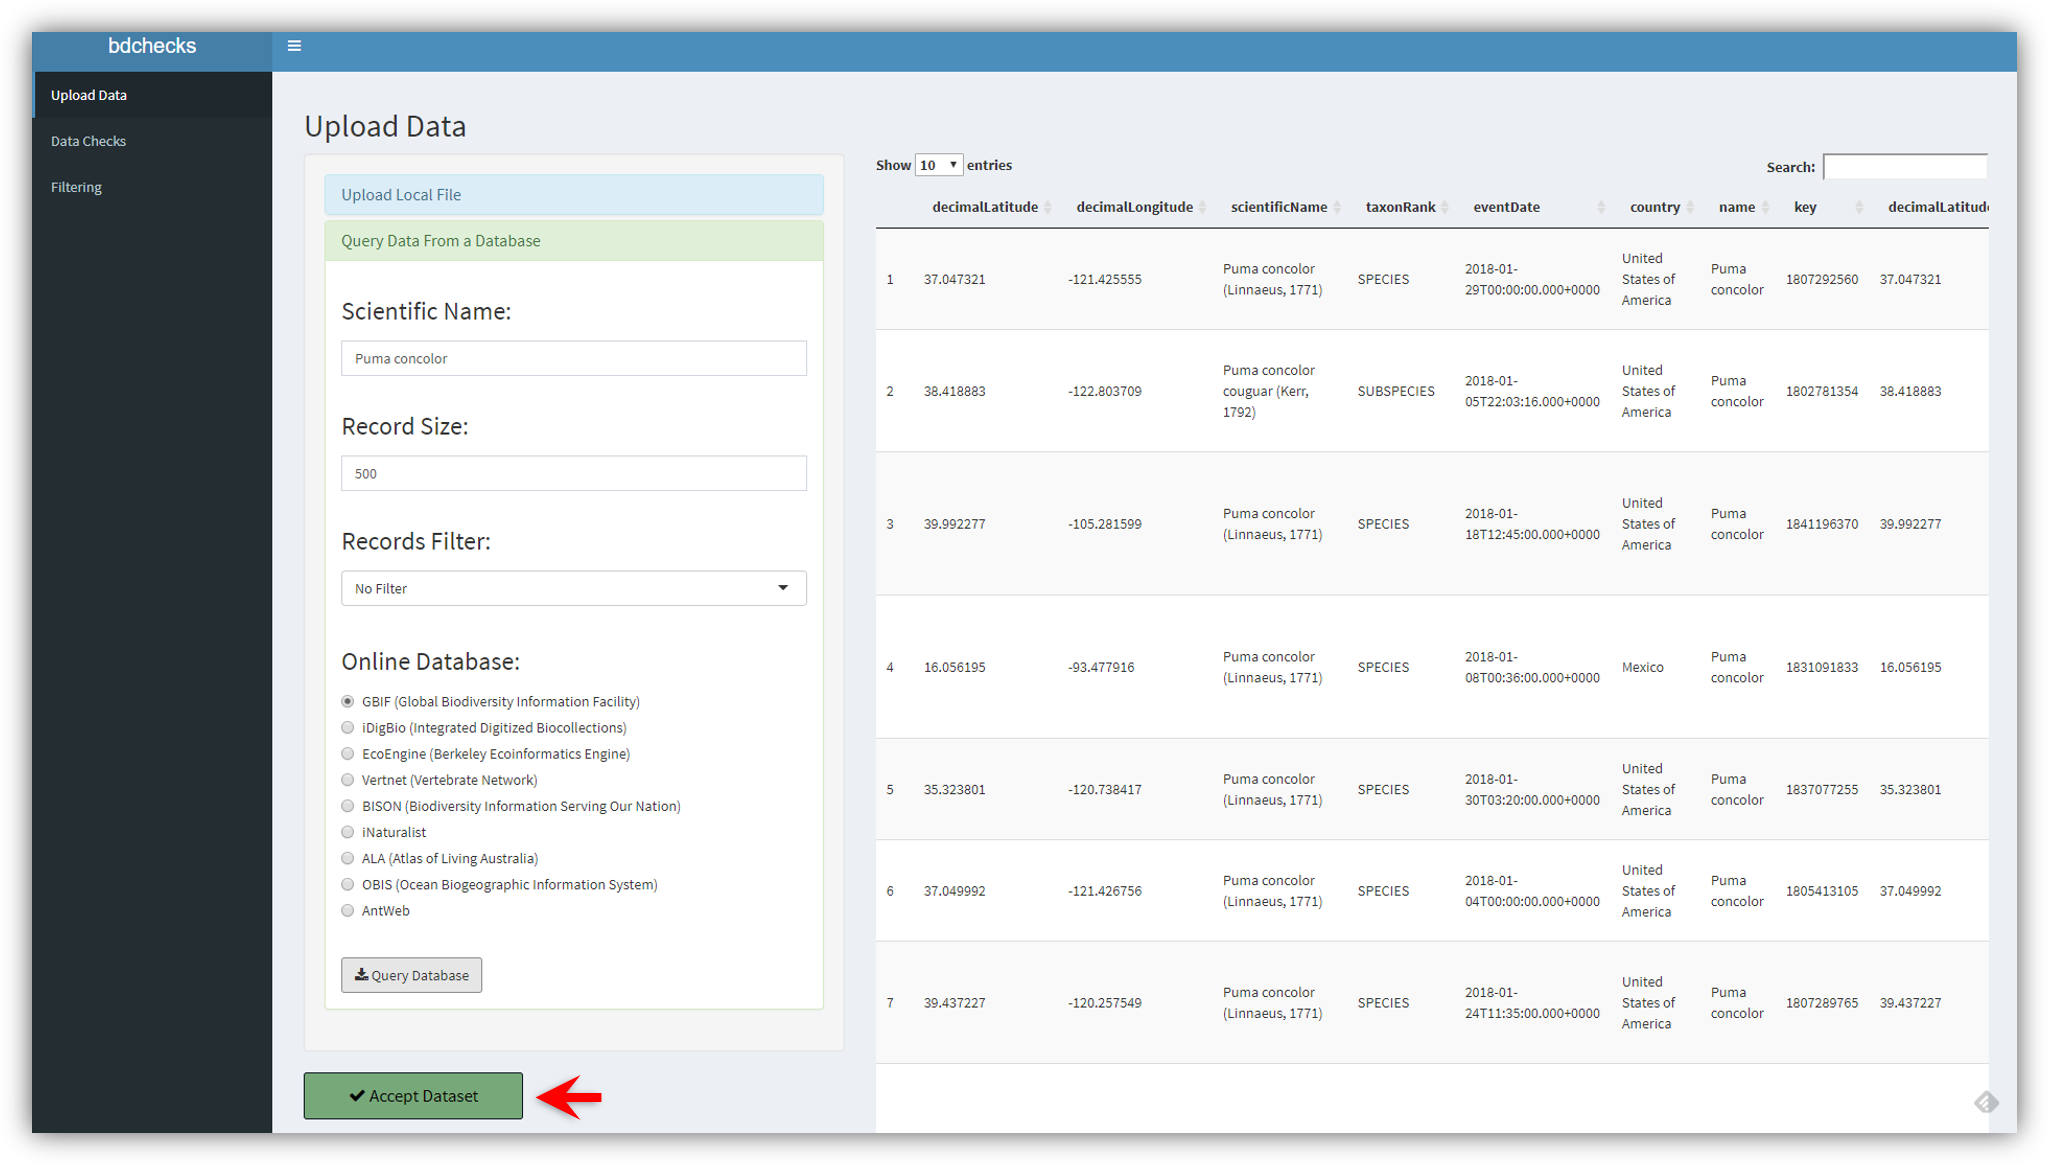
\includegraphics{img/bdchecks_accept_dataset.png}
\caption{`Accept dataset' to move to the next step}
\end{figure}

\section{Choose data checks}\label{choose-data-checks}

\begin{figure}
\centering
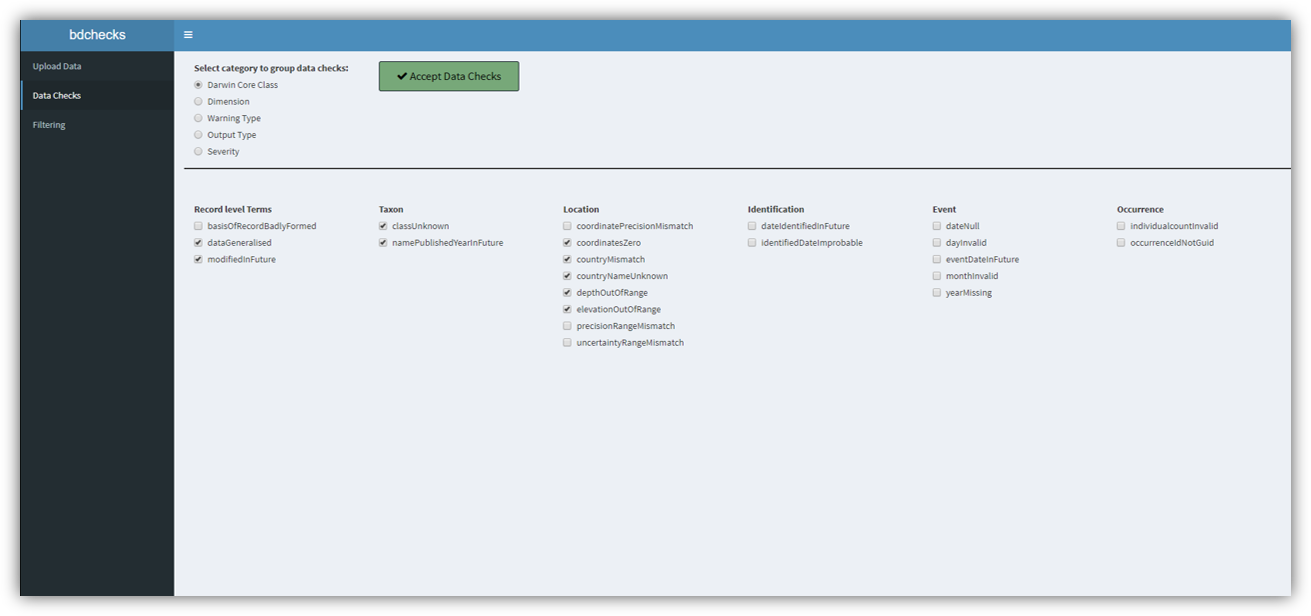
\includegraphics{img/bdchecks_choose_DC.png}
\caption{Choose a data check by checking its box}
\end{figure}

\begin{figure}
\centering
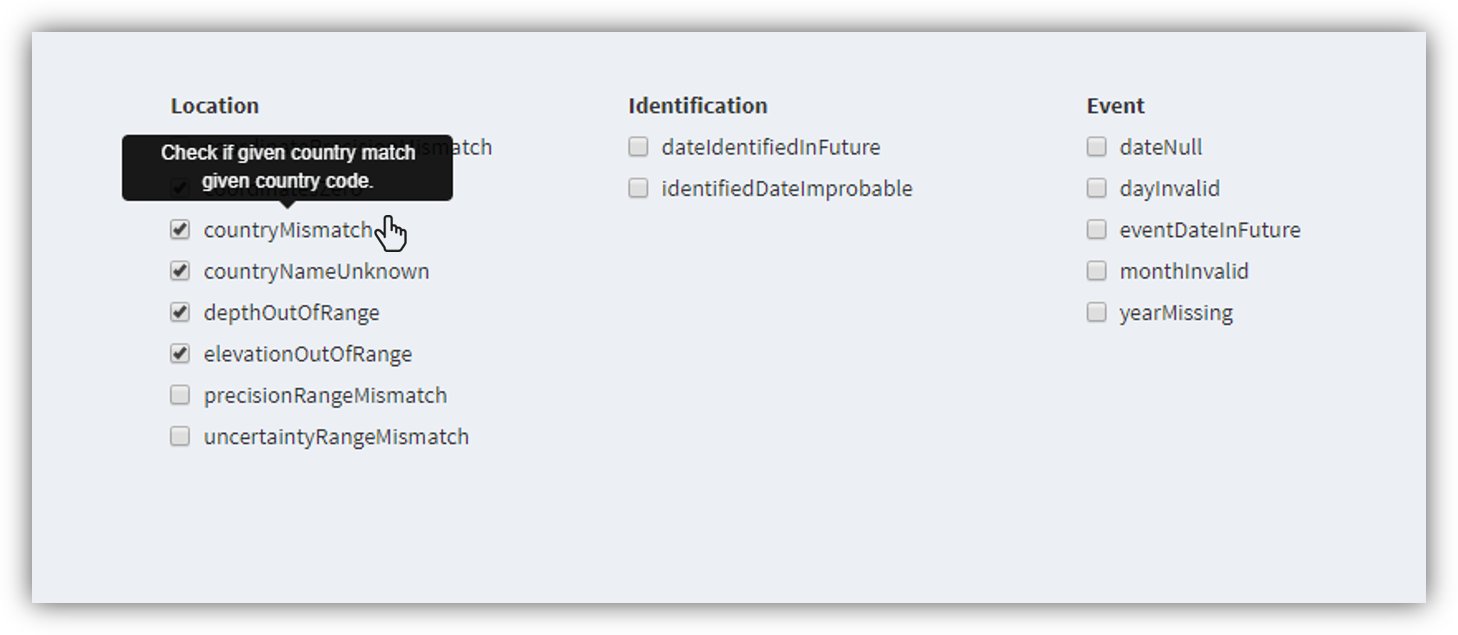
\includegraphics{img/bdchecks_hover.png}
\caption{Hovering over a data check name shows a short description}
\end{figure}

\section{Checks results and data
filtering}\label{checks-results-and-data-filtering}

\subsection{Overwiew}\label{overwiew}

\begin{figure}
\centering
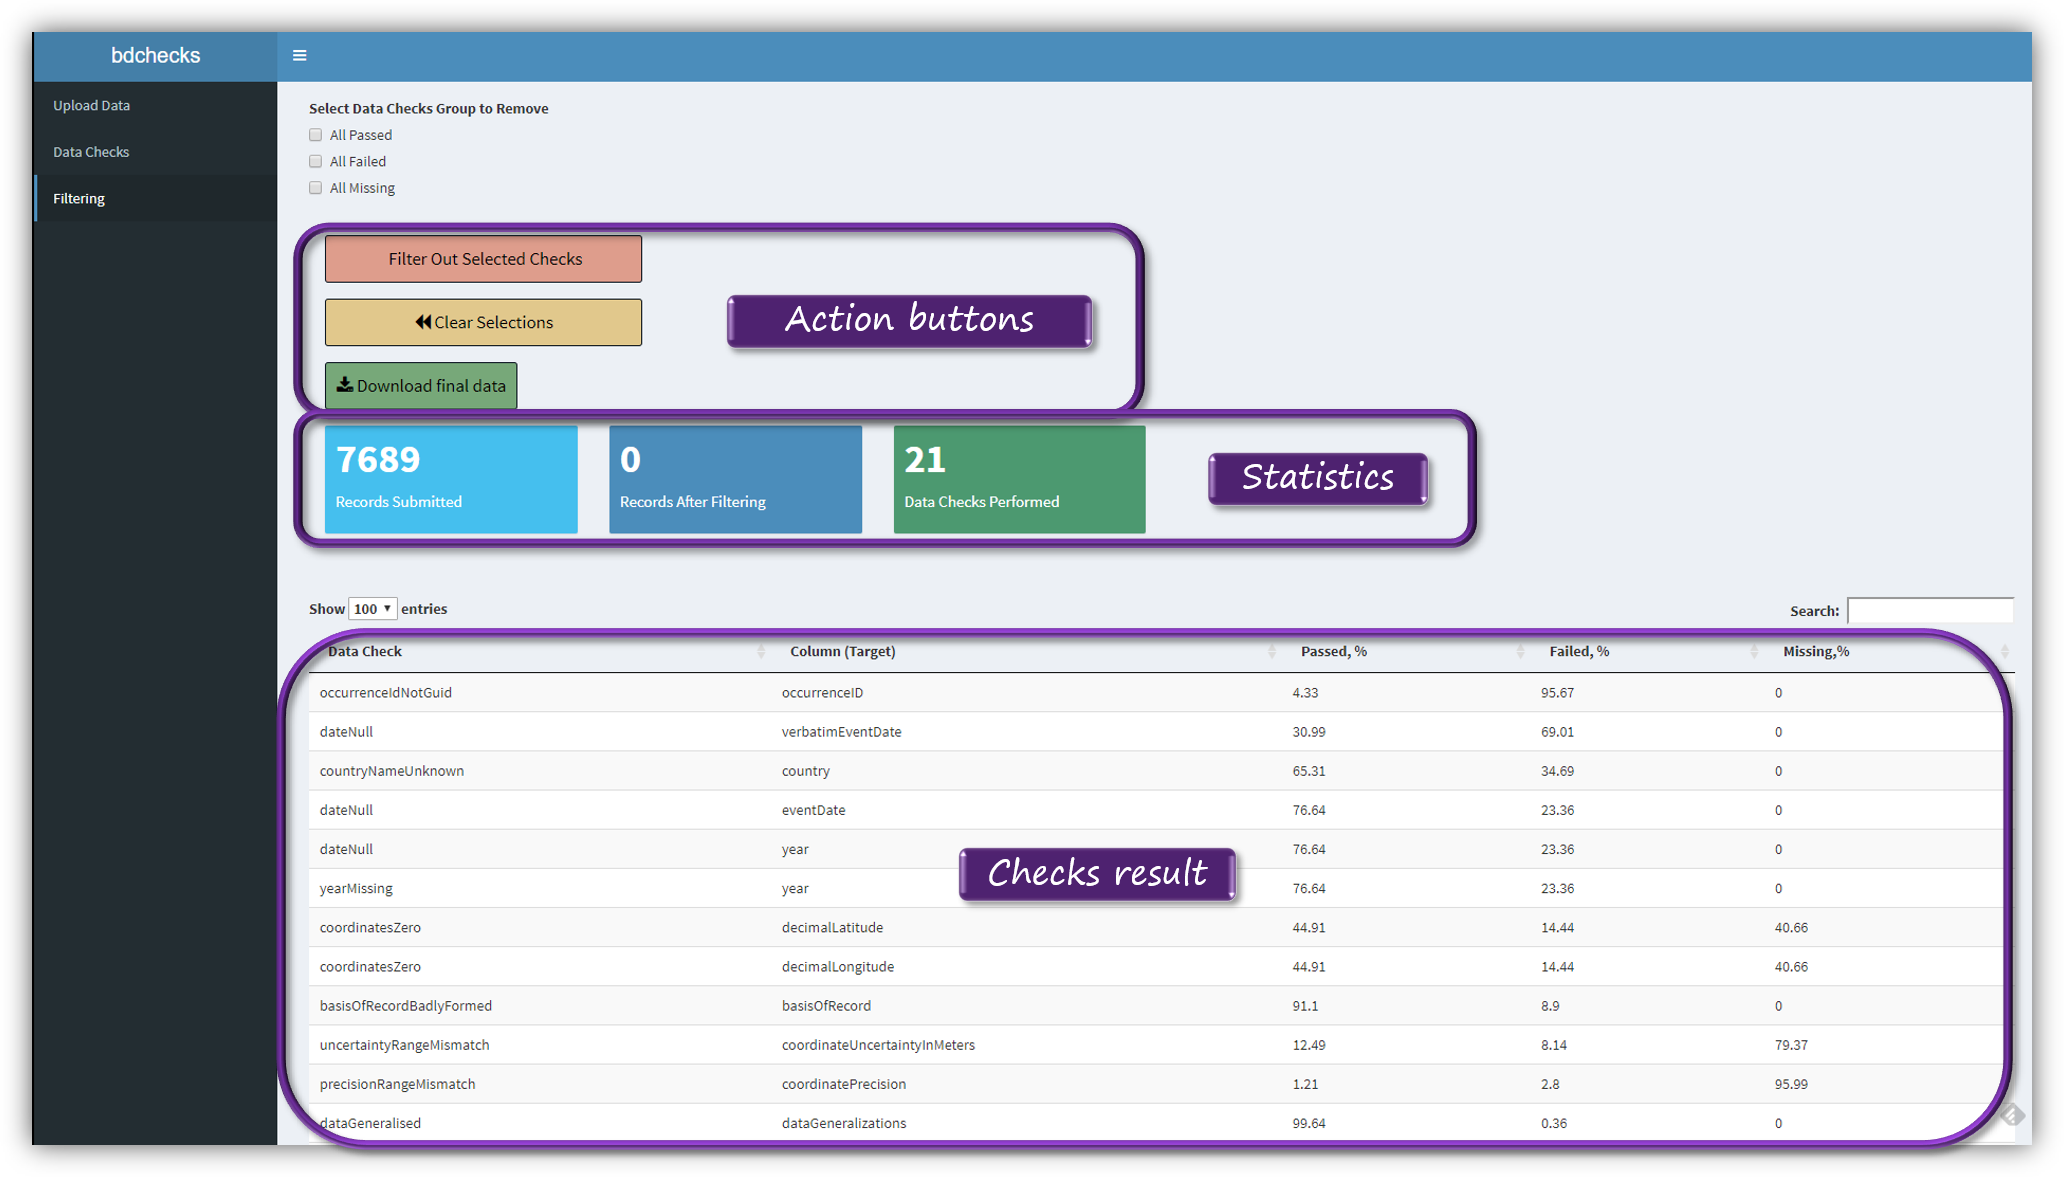
\includegraphics{img/bdchecks_DC_results_overview.png}
\caption{Results page overview}
\end{figure}

\subsection{Filtering the data based on the
results}\label{filtering-the-data-based-on-the-results}

\begin{figure}
\centering
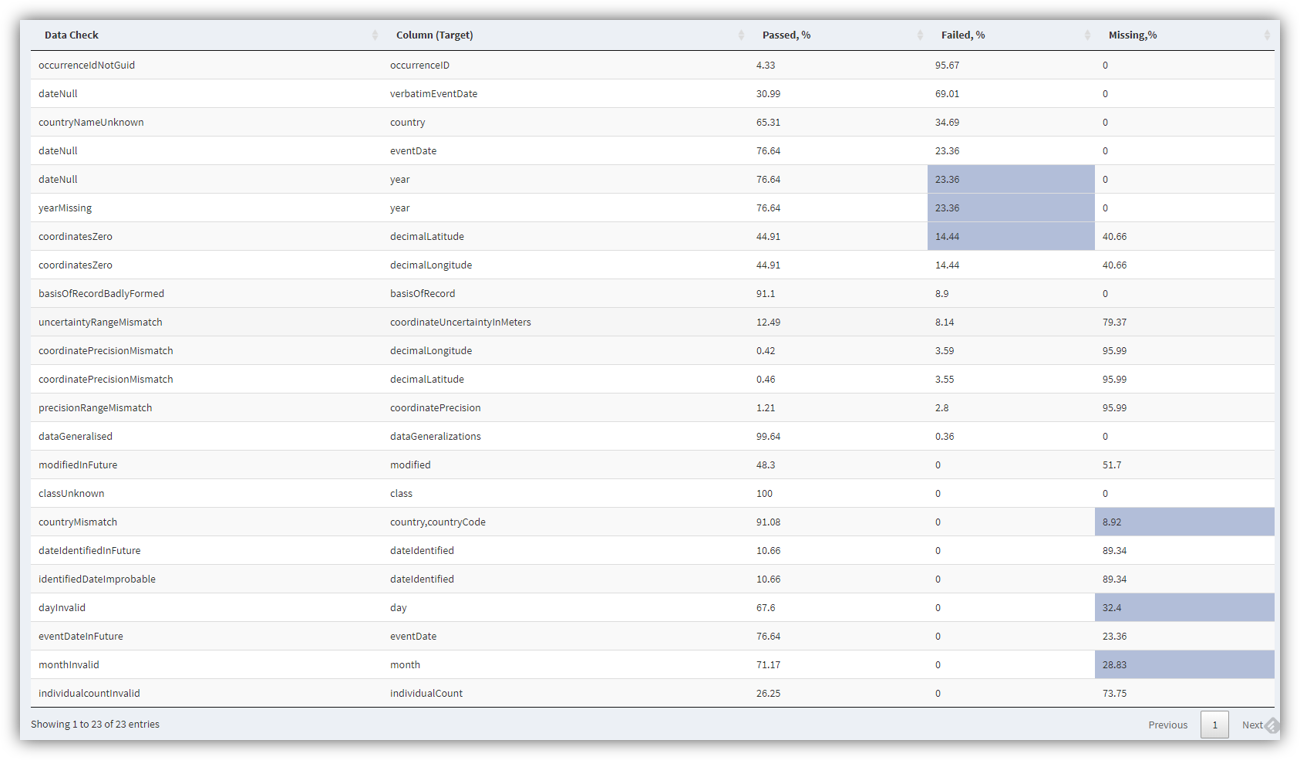
\includegraphics{img/bdchecks_filtering_table.png}
\caption{Choose specific results to filter out}
\end{figure}

\begin{figure}
\centering
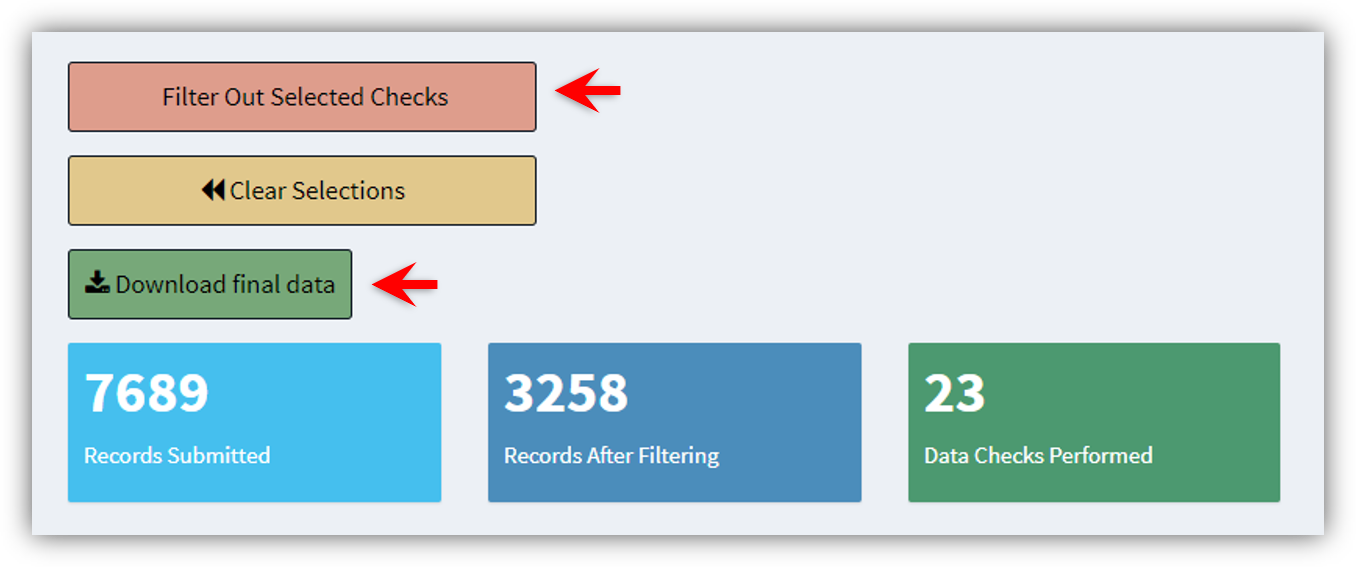
\includegraphics{img/bdchecks_filtering_action.png}
\caption{Filter the data and download your filtered data}
\end{figure}

\section{Closing the app}\label{closing-the-app}

Just close the app browser tab, and the R session will be terminated. To
reopen it run in the R Console \texttt{runbdchecks()}.

\section{References}\label{references}

\hypertarget{command-line-operations}{\chapter{Command line
operations}\label{command-line-operations}}

\begin{center}\rule{0.5\linewidth}{\linethickness}\end{center}

\section{Load package}\label{load-package}

Load the \texttt{bdchecks} package

\begin{Shaded}
\begin{Highlighting}[]
    \KeywordTok{library}\NormalTok{(bdchecks)}
\end{Highlighting}
\end{Shaded}

\section{Perform data checks}\label{perform-data-checks}

\texttt{bdchecks} contains a dataset on bats named \texttt{dataBats}.

To perform all data checks use \texttt{performDataCheck}:

\begin{Shaded}
\begin{Highlighting}[]
\NormalTok{resultDC <-}\StringTok{ }\NormalTok{bdchecks}\OperatorTok{::}\KeywordTok{performDataCheck}\NormalTok{(bdchecks}\OperatorTok{::}\NormalTok{dataBats)}
\end{Highlighting}
\end{Shaded}

replace \texttt{bdchecks::dataBats} with your own dataset name.

\section{Review performed checks}\label{review-performed-checks}

See which data checks were performed:

\begin{Shaded}
\begin{Highlighting}[]
\NormalTok{resultDC}
\end{Highlighting}
\end{Shaded}

Review data checks result (\% of records that passed, failed or have
missing data)

\begin{Shaded}
\begin{Highlighting}[]
\CommentTok{# Nice summary}
\KeywordTok{summary_DC}\NormalTok{(resultDC)}
\end{Highlighting}
\end{Shaded}

\section{Filtering your data}\label{filtering-your-data}

\textbf{{{[} TBA {]}}}

\hypertarget{data-checks-yaml-file}{\chapter{Data checks YAML
file}\label{data-checks-yaml-file}}

\begin{center}\rule{0.5\linewidth}{\linethickness}\end{center}

The YMAL file holds the code and metadata of all data checks. The checks
are derived from a core suite of tests and assertions being developed by
TDWG's Biodiversity Data Quality \textbf{Task Group 2 ( Data Quality
Tests and Assertions)}. More information and links can be found in the
\protect\hyperlink{learn-more}{Learn more} section.

\section{Data check example}\label{data-check-example}

\begin{verbatim}
DC_b23110e7-1be7-444a-a677-cdee0cf4330c:
  name: countryMismatch
  meta:
    Description:
      Main: Check if given country match given country code.
      InputQuestion: Does country and country code match?
      Example:
        Fail: Country name (dwc:country) and ISO country code (dwc:countryCode) do
          not match
        Pass: Country name (dwc:country) and ISO country code (dwc:countryCode) match
        InputFail: country=Australia, countryCode=4
        InputPass: country=Australia, countryCode=AU
        OutputFail: Failed
        OutputPass: Passed
      Resolution:
        Record: SingleRecord
        Term: MultiTerm
      DarwinCoreClass: Location
      Keywords: location,iso,country
      guid: b23110e7-1be7-444a-a677-cdee0cf4330c
    Flags:
      Severity: Warning
      Warning: Inconsistent
      Output: Validation
      Dimension: Consistency
    Pseudocode: |
      get.Country($countryCode) == $country
    Source:
      Reference:
      CreatedBy: Povilas Gibas
      MaintainedBy: Povilas Gibas
      CreationDate: 2018-06-27
      ModificationDate: 2018-06-27
      ModificationHist:
  Input:
    Target: country,countryCode
    Dependency:
      DependencyType: Internal
      DataChecks:
      Rpackages: rgbif 
      Data: isocodes$name,isocodes$code
  Functionality: |
      FUNC <- function() {
          result <- sapply(seq_along(TARGET1), function(i) {
              if (is.na(TARGET1[i]) | is.na(TARGET2[i])) {
                  NA
              } else {
                  which(DEPEND1 == TARGET1[i]) == which(DEPEND2 == TARGET2[i])
              }
          })
          result <- unlist(result)
          return(result)
       }
\end{verbatim}

\section{Manage your own data checks}\label{manage-your-own-data-checks}

After adding/ removing/ editing the YAML file, you can load data checks
into R using \texttt{getDC()} function.

\begin{Shaded}
\begin{Highlighting}[]
\NormalTok{DC <-}\StringTok{ }\KeywordTok{getDC}\NormalTok{(}\StringTok{"path to your YAML file"}\NormalTok{)}
\end{Highlighting}
\end{Shaded}

You can also export data checks from your YAML file to .rda and roxygen2
comments.

\begin{Shaded}
\begin{Highlighting}[]
\KeywordTok{exportDC}\NormalTok{(}\StringTok{"path to your YAML file"}\NormalTok{)}
\end{Highlighting}
\end{Shaded}

\chapter{\texorpdfstring{\texttt{bdchecks}
architecture}{bdchecks architecture}}\label{bdchecks-architecture}

\begin{center}\rule{0.5\linewidth}{\linethickness}\end{center}

\section{The overall architecture}\label{the-overall-architecture}

\textbf{{{[} TBA {]}}}

\section{Component 1****}\label{component-1}

\textbf{{{[} TBA {]}}}

\section{Component 2****}\label{component-2}

\textbf{{{[} TBA {]}}}

\chapter{Getting your feedback}\label{getting-your-feedback}

\begin{center}\rule{0.5\linewidth}{\linethickness}\end{center}

Loading\ldots{}

\section{Report a bug}\label{report-a-bug}

Submit an issue at \url{https://github.com/bd-R/bdchecks/issues}

\section{Contribute}\label{contribute}

Contribute: \url{https://github.com/bd-R/bdchecks}

Join: \url{https://bd-r-group.slack.com}

\chapter{\texorpdfstring{\texttt{bdchecks}
citation}{bdchecks citation}}\label{bdchecks-citation}

\begin{center}\rule{0.5\linewidth}{\linethickness}\end{center}

\begin{Shaded}
\begin{Highlighting}[]
\KeywordTok{citation}\NormalTok{(}\StringTok{"bdchecks"}\NormalTok{)}
\end{Highlighting}
\end{Shaded}

\begin{verbatim}
## 
## To cite package 'bdchecks' in publications use:
## 
##   Povilas Gibas, Tomer Gueta, Vijay Barve, Thiloshon Nagarajah and
##   Yohay Carmel (2018). bdchecks: Biodiversity Data Checks. R
##   package version 0.1.2. https://github.com/bd-R/bdchecks
## 
## A BibTeX entry for LaTeX users is
## 
##   @Manual{,
##     title = {bdchecks: Biodiversity Data Checks},
##     author = {Povilas Gibas and Tomer Gueta and Vijay Barve and Thiloshon Nagarajah and Yohay Carmel},
##     year = {2018},
##     note = {R package version 0.1.2},
##     url = {https://github.com/bd-R/bdchecks},
##   }
\end{verbatim}

\hypertarget{learn-more}{\chapter{Learn more}\label{learn-more}}

\begin{center}\rule{0.5\linewidth}{\linethickness}\end{center}

\begin{itemize}
\item
  \textbf{TDWG's data quality tests and assertions Task Group}
\item
  \textbf{Core suite of tests and assertions}
\item
  \textbf{Core tests and assertions as GitHub issues}
\item
  \textbf{A conceptual framework for quality assessment and management
  of biodiversity data \citep{Veiga2017} }
\end{itemize}

\subsubsection*{References}\label{references-1}
\addcontentsline{toc}{subsubsection}{References}

\bibliography{bib/book.bib,bib/DarwinCloud.bib,bib/DwC-paper.bib,bib/Veiga-2017.bib}


\end{document}
